%%%%%%%%%%%%%%
%% Run LaTeX on this file several times to get Table of Contents,
%% cross-references, and citations.

%% If you have font problems, you may edit the w-bookps.sty file
%% to customize the font names to match those on your system.

%% w-bksamp.tex. Current Version: Feb 16, 2012
%%%%%%%%%%%%%%%%%%%%%%%%%%%%%%%%%%%%%%%%%%%%%%%%%%%%%%%%%%%%%%%%
%
%  Sample file for
%  Wiley Book Style, Design No.: SD 001B, 7x10
%  Wiley Book Style, Design No.: SD 004B, 6x9
%
%
%  Prepared by Amy Hendrickson, TeXnology Inc.
%  http://www.texnology.com
%%%%%%%%%%%%%%%%%%%%%%%%%%%%%%%%%%%%%%%%%%%%%%%%%%%%%%%%%%%%%%%%

%%%%%%%%%%%%%
% 7x10
%\documentclass{wileySev}

% 6x9
\documentclass{wileySix}

\usepackage{graphicx}
\usepackage{array}

%%%%%%%
%% for times math: However, this package disables bold math (!)
%% \mathbf{x} will still work, but you will not have bold math
%% in section heads or chapter titles. If you don't use math
%% in those environments, mathptmx might be a good choice.

% \usepackage{mathptmx}

% For PostScript text
\usepackage{w-bookps}

%%%%%%%%%%%%%%%%%%%%%%%%%%%%%%%%%%%%%%%%%%%%%%%%%%%%%%%%%%%%%%%%
%% Other packages you might want to use:

% for chapter bibliography made with BibTeX
% \usepackage{chapterbib}

% for multiple indices
% \usepackage{multind}

% for answers to problems
% \usepackage{answers}

%%%%%%%%%%%%%%%%%%%%%%%%%%%%%%
%% Change options here if you want:
%%
%% How many levels of section head would you like numbered?
%% 0= no section numbers, 1= section, 2= subsection, 3= subsubsection
%%==>>
\setcounter{secnumdepth}{3}

%% How many levels of section head would you like to appear in the
%% Table of Contents?
%% 0= chapter titles, 1= section titles, 2= subsection titles,
%% 3= subsubsection titles.
%%==>>
\setcounter{tocdepth}{2}

%% Cropmarks? good for final page makeup
%% \docropmarks

%%%%%%%%%%%%%%%%%%%%%%%%%%%%%%
%
% DRAFT
%
% Uncomment to get double spacing between lines, current date and time
% printed at bottom of page.
% \draft
% (If you want to keep tables from becoming double spaced also uncomment
% this):
% \renewcommand{\arraystretch}{0.6}
%%%%%%%%%%%%%%%%%%%%%%%%%%%%%%

%%%%%%% Demo of section head containing sample macro:
%% To get a macro to expand correctly in a section head, with upper and
%% lower case math, put the definition and set the box
%% before \begin{document}, so that when it appears in the
%% table of contents it will also work:

\newcommand{\VT}[1]{\ensuremath{{V_{T#1}}}}

%% use a box to expand the macro before we put it into the section head:

\newbox\sectsavebox
\setbox\sectsavebox=\hbox{\boldmath\VT{xyz}}

%%%%%%%%%%%%%%%%% End Demo


\begin{document}


\booktitle{Belajar Phalcon}
\subtitle{Buku Phalcon Untuk Pemula}

\authors{Rolly M. Awangga\\
\affil{Politeknik Pos Indonesia}
}

\offprintinfo{Belajar Phalcon, First Edition}{Rolly M. Awangga}

%% Can use \\ if title, and edition are too wide, ie,
%% \offprintinfo{Survey Methodology,\\ Second Edition}{Robert M. Groves}

%%%%%%%%%%%%%%%%%%%%%%%%%%%%%%
%%
\halftitlepage

\titlepage


\begin{copyrightpage}{2007}
Survey Methodology / Robert M. Groves . . . [et al.].
\       p. cm.---(Wiley series in survey methodology)
\    ``Wiley-Interscience."
\    Includes bibliographical references and index.
\    ISBN 0-471-48348-6 (pbk.)
\    1. Surveys---Methodology.  2. Social
\  sciences---Research---Statistical methods.  I. Groves, Robert M.  II. %
Series.\\

HA31.2.S873 2007
001.4'33---dc22                                             2004044064
\end{copyrightpage}



\dedication{To my parents}

\begin{contributors}
\name{Masayki Abe,} Fujitsu Laboratories Ltd., Fujitsu Limited, Atsugi,
Japan

\name{L. A. Akers,} Center for Solid State Electronics Research, Arizona
State University, Tempe, Arizona

\name{G. H. Bernstein,} Department of Electrical and
Computer Engineering, University of Notre Dame, Notre Dame, South Bend,
Indiana; formerly of
Center for Solid State Electronics Research, Arizona
State University, Tempe, Arizona
\end{contributors}

\contentsinbrief
\tableofcontents
\listoffigures
\listoftables


\begin{foreword}
This is the foreword to the book.
\end{foreword}

\begin{preface}
This is an example preface.
This is an example preface.
This is an example preface.
This is an example preface.

\prefaceauthor{R. K. Watts}
\where{Durham, North Carolina\\
September, 2007}

\end{preface}


\begin{acknowledgments}
From Dr.~Jay Young, consultant from Silver Spring, Maryland, I received
the initial push to even consider writing this book. Jay was a constant
``peer reader'' and very welcome advisor durying this year-long process.


To all these wonderful people I owe a deep sense of gratitude especially now
that this project has been completed.
\authorinitials{G. T. S.}
\end{acknowledgments}

\begin{acronyms}
\acro{ACGIH}{American Conference of Governmental Industrial Hygienists}
\acro{AEC}{Atomic Energy Commission}
\acro{OSHA}{Occupational Health and Safety Commission}
\acro{SAMA}{Scientific Apparatus Makers Association}
\end{acronyms}

\begin{glossary}
\term{NormGibbs}Draw a sample from a posterior distribution
of data with an unknown mean and variance using Gibbs sampling.

\term{pNull}Test a one sided hypothesis from a numberically
specified posterior CDF or from a sample from the posterior

\term{sintegral}A numerical integration using Simpson's rule
\end{glossary}

\begin{symbols}
\term{A}Amplitude

\term{\hbox{\&}}Propositional logic symbol

\term{a}Filter Coefficient

\bigskip

\term{\mathcal{B}}Number of Beats
\end{symbols}

\begin{introduction}

%% optional, but if you want to list author:

\introauthor{Catherine Clark, PhD.}
{Harvard School of Public Health\\
Boston, MA, USA}

The era of modern \index{microelectronics}\index{microelectronics!modern}
began in 1958 with the invention of the
integrated circuit by J.~S.~Kilby
 of Texas Instruments \cite{kilby}.
His first chip is shown in Fig.~I. For comparison,
Fig.~I.2 shows a modern microprocessor chip, \cite{beren}.


This is the introduction.
This is the introduction.
This is the introduction.
This is the introduction.
This is the introduction.
This is the introduction.

\begin{equation}
ABC {\cal DEF} \alpha\beta\Gamma\Delta\sum^{abc}_{def}
\end{equation}


\begin{chapreferences}{3.}
\bibitem{zkilby}J. S. Kilby,
``Invention of the Integrated Circuit,'' {\it IEEE Trans. Electron Devices,}
{\bf ED-23,} 648 (1976).

\bibitem{zhamming}R. W. Hamming,
                 {\it Numerical Methods for Scientists and
                 Engineers}, Chapter N-1, McGraw-Hill,
                 New York, 1962.

\bibitem{zHu}J. Lee, K. Mayaram, and C. Hu, ``A Theoretical
               Study of Gate/Drain Offset in LDD MOSFETs''
                     {\it IEEE Electron Device Lett.,} {\bf EDL-7}(3). 152
                     (1986).
\end{chapreferences}
\end{introduction}


\chapter[Phalcon - Overview]
{Phalcon -\\ Overview}
\section{Pengenalan}
Phalcon diperkenalkan sebagai salah satu Framework PHP terbaru, yang dikembangkan oleh sekelompok pengembang yang antusias. Phalcon adalah Framework yang digabungkan secara longgar, yang berarti memungkinkannya bisa membuat komponen objek menempel seperti lem, berdasarkan kebutuhan aplikasi.

Phalcon memberikan beberapa fitur yang unik sebagai keunggulan dibandingkan framework yang lain (baik framework tradisional atau yang sering dipakai) di pemrograman PHP. Diantaranya:

\begin{itemize}
 \item Framework yang full-stack open source

 \item User hanya membutuhkan code yang lebih sedikit untuk mendapatkan keuntungan di beberapa komponen

 \item bisa dipakai untuk membuat framework independen seperti yang dibutuhkan. Contohnya, jika kita hanya membutuhkan komponen cache yang dimiliki Phalcon, kita bisa menggunakannya di aplikasi apapun baik yang dibuat PHP atau menggunakan framework lain.

 \item Di sisi developer, mereka memounyai konsep MVC (Model-View-Controller) dan ORM (Object-Relational Modeling), bekerja dengan mudahnya dalam pemrograman Phalcon.
 \end{itemize}

\subsection{Performance}

Perbedaan Framework Phalcon dengan Framework Yii dan Laravel

\begin{center}
 \begin{tabular}{ | m{2em} | m{3cm}| m{3cm} | m{3cm} }
 \hline
 - & Yii & Laravel & Phalcon \\ [0.5ex]
 \hline\hline
 Tipe dalam Proyek & Yii adalah spesialis membuat proyek skala besar seperti forums, portals, CMS, RESTful web services, dll. & Laravel biasa digunakan untuk aplikasi berbasis web, laravel terkenal karena sintaks nya yang sangat indah dan canggih & Phalcon diguakan untuk semua variasi proyek \\
 \hline
 Database yang Mendukung & Yii mendukung semua RDBMS dan non-RDBMS & Laravel mendukung semua RDBMS & Phalcon memberikan dukungan secara equal (sama) baik RDBMS maupun non-RDBMS \\
 \hline
 Bahasa Pemrograman & Framework Yii menggunakan bahasa pemrograman PHP saja & Laravel menggunakan bahasa pemrograman PHP dan mengikuti pattern MVC & Phalcon menggunakan bahasa pemrograman PHP dan C \\
 \hline
 Keterjangkauan & Yii cukup baik di gunakan di skala proyek kecil ke menengah & Laravel punya keterjangkauan yang tinggi dalam skala proyek & Phalcon cocok untuk proyek skala menengah \\
 \hline
 Performa & Sedikit lambat & Performa tinggi namun masih dibawah Phalcon & Performa Tinggi \\ [1ex]
 \hline
\end{tabular}
\end{center}


\subsubsection{This is the subsubsection}
Here is some text after the subsubsection.
Here is some text after the subsubsection.
Here is some text after the subsubsection.
Here is some text after the subsubsection.

\paragraph{This is the paragraph}
Here is some normal text.
Here is some normal text.
Here is some normal text.
Here is some normal text.

\section{Tips On Special Section Heads}
Here are some things you can do for a special
section head.

\section[This Version of Section Head will be sent Contents]
{Break Long Section heads\\ with double backslash}
Here is some normal text.
Here is some normal text.
Here is some normal text.

 \section[This show how to explicitly break lines
\string\hfill\string\break\space in Table of Contents]
{Here is a Section Title}
See this section head for information on how to explicitly break lines in
table of contents.

\section{How to get \lowercase{lower case} in section head: \lowercase{$p$}$H$}
Here is some normal text.
Here is some normal text.
Here is some normal text.

\section{How to use a macro that has both upper and lower case parts:
\copy\sectsavebox}
See the top of this file where the definition and box were set.

%% Sending different version of section to running head,
%% so that the size of math is correct in running head:
\markright{Sample macro \VT{\lowercase{xyz}} sent to running head}

\section{Equation}

For optimal vertical spacing, no blank lines before or after
equations
\begin{equation}
\alpha\beta\Gamma\Delta
\end{equation}
as you see here.


\chapter{Enviromental Setup}
}

\section{Aplikasi yang dibutuhkan}
Memerlukan XAMPP untuk instalasi Framework Phalcon.
\begin{itemize}
 \item Step 1: Download Install lah file DLL (Dynamic Link Library) Phalcon di link https://phalconphp.com/en/download, sesuaikan file dll nya dengan konfigurasi versi XAMPP Anda.
 \item Step 2: Extract phalcon-php.dll file ke direktori /php/ext di folder XAMPP.
 \item Step 3: Edit file php.ini didalam folder /XAMPP/php/php.ini. Tambahkan "extension=php\_phalcon.dll" tanpa tanda kutip ke baris akhir php.ini.
 \item Step 4:
 \item Step 5:
 \item Step 6:
 \item Step 7:
 \item Step 8:
 \end{itemize}
 
  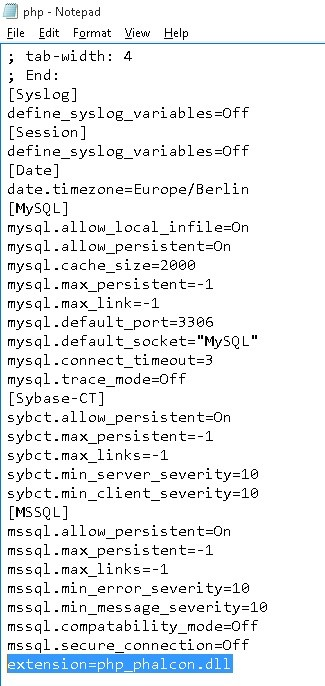
\includegraphics[scale=0.8]{extension}
  
  Gambar dari Step 2: Yang harus ditambahkan di file php.ini


\chapter{Second Edited Book Sample Chapter Title}
\chapterauthors{George Smeal, Ph.D.\affilmark{1}, Sally Smith,
M.D.\affilmark{2} and Stanley Kubrick\affilmark{1}
\chapteraffil{\affilmark{1}AT\&T Bell Laboratories
Murray Hill, New Jersey\\
\affilmark{2}Harvard Medical School,
Boston, Massachusetts}
}

\section{Sample Section}
Here is some sample text.

\newpage

\section{Example, Figure and Tables}
\vskip6pt
\begin{example}[Optional Example Name]
Use Black's law [Equation (6.3)] to estimate the reduction in useful product
life if a metal line is initially run at 55$^\circ$C at a maximum line
current density.
\end{example}




\begin{figure}[ht]
illustration here
%\centerline{\includegraphics[width=.5\textwidth]{filename}}
\caption{Short figure caption.}
\end{figure}

\begin{figure}[ht]
\vskip2pt
\caption{Oscillograph for  memory address access operations,
showing 500 ps
address access time and superimposed signals
of address access in 1 kbit
memory plane.}
\end{figure}

\begin{table}[ht]
\caption{Small Table}
\centering
\begin{tabular}{cccc}
\hline
one&two&three&four\\
\hline
C&D&E&F\\
\hline
\end{tabular}
\end{table}



\begin{table}[ht]
\caption{Effects of the two types of $\alpha\beta\sum^A_B$ scaling proposed by Dennard \newline
and
co-workers$^{a,b}$}
\begin{tabular*}{\textwidth}{@{\extracolsep{\fill}}lcc}
\hline
Parameter& $\kappa$ Scaling & $\kappa$, $\lambda$ Scaling\cr
\hline
Dimension&$\kappa^{-1}$&$\lambda^{-1}$\cr
Voltage&$\kappa^{-1}$&$\kappa^{-1}$\cr
Currant&$\kappa^{-1}$&$\lambda/\kappa^{2}$\cr
Dopant Concentration&$\kappa$&$\lambda^2/\kappa$\cr
\hline
\end{tabular*}
\begin{tablenotes}
$^a$Refs.~19 and 20.

$^b\kappa, \lambda>1$.
\end{tablenotes}
\end{table}

\subsection{Side by Side Tables and Figures}

\begin{figure}[ht]
\sidebyside{
Space for figure...
\caption{This caption will go on the left side of
the page. It is the initial caption of two side-by-side captions.}
}
{
Space for second figure...
\caption{This caption will go on the right side of
the page. It is the second of two side-by-side captions.}
}
\end{figure}


The command \verb+\sidebyside{}{}+ works similarly for tables:

 \begin{table}[ht]
 \sidebyside{
\caption{Table Caption}
\begin{tabular}{cccc}
one&two&three&four\\
a &little&sample&table
\end{tabular}
}
 {
\caption{Table Caption}
\begin{tabular}{cccc}
A&B&C&D\\
a &second little& sample&table
\end{tabular}
}
 \end{table}


When using \verb+\sidebyside+, one must
use the cross referencing command \verb+\label{}+ after and  {\it outside}
 of \verb+\caption{}+:

\begin{verbatim}
 \begin{table}
 \sidebyside{\caption{Table Caption}\label{tab1}
 first table}
 {\caption{Table Caption}\label{tab2} second table}
 \end{table}
\end{verbatim}
 or,
\begin{verbatim}
 \begin{figure}
 \sidebyside{\vskip<dimen>\caption{fig caption}\label{fig1}}
 {\vskip<dimen>\caption{fig caption}\label{fig2}}
 \end{figure}
\end{verbatim}





\section{Algorithm}
This is a sample algorithm.

\begin{algorithm}
{\bf state\_transition algorithm} $\{$
\        for each neuron $j\in\{0,1,\ldots,M-1\}$
\        $\{$
\            calculate the weighted sum $S_j$ using Eq. (6);
\            if ($S_j>t_j$)
\                    $\{$turn ON neuron; $Y_1=+1\}$
\            else if ($S_j<t_j$)
\                    $\{$turn OFF neuron; $Y_1=-1\}$
\            else
\                    $\{$no change in neuron state; $y_j$ remains %
unchanged;$\}$
\        $\}$
$\}$
\end{algorithm}

Here is some normal text.
Here is some normal text.
Here is some normal text.
Here is some normal text.
Here is some normal text.
Here is some normal text.
Here is some normal text.
Here is some normal text.
Here is some normal text.
Here is some normal text.
Here is some normal text.
Here is some normal text.
Here is some normal text.
Here is some normal text.


\begin{quote}
This is a sample of extract or quotation.
This is a sample of extract or quotation.
This is a sample of extract or quotation.
\end{quote}

\begin{enumerate}
\item
This is the first item in the numbered list.

\item
This is the second item in the numbered list.
This is the second item in the numbered list.
This is the second item in the numbered list.
\end{enumerate}

\begin{itemize}
\item
This is the first item in the itemized list.

\item
This is the first item in the itemized list.
This is the first item in the itemized list.
This is the first item in the itemized list.
\end{itemize}

\begin{itemize}
\item[]
This is the first item in the itemized list.

\item[]
This is the first item in the itemized list.
This is the first item in the itemized list.
This is the first item in the itemized list.
\end{itemize}

\begin{problems}
\prob
For Hooker's data, Problem 1.2, use the Box and Cox and Atkinson procedures to determine a appropriate transformation of PRES
in the regression of PRES on TEMP. find $\hat\lambda$, $\tilde\lambda$,
the score test, and the added variable plot for the score.
Summarize the results.

\prob
The following data were collected in a study of the effect of dissolved sulfur
on the surface tension of liquid copper (Baes and Killogg, 1953).

{\centering
\vskip6pt
\begin{tabular}{rlcc}
\hline
&&\multicolumn2c{$Y$= Decrease in Surface Tension}\\
\multicolumn2c{$x$ = Weight \% sulfur}
&\multicolumn2c{(dynes/cm), two Replicates}\\
\hline
0.&034&301&316\\
0.&093&430&422\\
0.&30&593&586\\
\hline
\end{tabular}
\vskip6pt
}


\subprob
Find the transformations of $X$ and $Y$ sot that in the transformed scale
the regression is linear.

\subprob
Assuming that $X$ is transformed to $\ln(X)$, which choice of $Y$ gives
better results,
$Y$ or $\ln(Y)$? (Sclove, 1972).

\sidebysidesubprob{In the case of $\alpha_1$?}{In the case of $\alpha_2$?}

\prob
Examine the Longley data, Problem 3.3, for applicability of assumptions of the
linear model.

\sidebysideprob{In the case of $\Gamma_1$?}{In the case of $\Gamma_2$?}

\end{problems}


\begin{exercises}
\exer
For Hooker's data, Exercise 1.2, use the Box and Cox and Atkinson procedures to determine a appropriate transformation of PRES
in the regression of PRES on TEMP. find $\hat\lambda$, $\tilde\lambda$,
the score test, and the added variable plot for the score.
Summarize the results.

\exer
The following data were collected in a study of the effect of dissolved sulfur
on the surface tension of liquid copper (Baes and Killogg, 1953).

{\centering
\vskip6pt
\begin{tabular}{rlcc}
\hline
&&\multicolumn2c{$Y$= Decrease in Surface Tension}\\
\multicolumn2c{$x$ = Weight \% sulfur}
&\multicolumn2c{(dynes/cm), two Replicates}\\
\hline
0.&034&301&316\\
0.&093&430&422\\
0.&30&593&586\\
\hline
\end{tabular}
\vskip6pt
}


\subexer
Find the transformations of $X$ and $Y$ sot that in the transformed scale
the regression is linear.

\subexer
Assuming that $X$ is transformed to $\ln(X)$, which choice of $Y$ gives
better results,
$Y$ or $\ln(Y)$? (Sclove, 1972).

\sidebysidesubexer{In the case of $\Delta_1$?}{In the case of $\Delta_2$?}

\exer
Examine the Longley data, Problem 3.3, for applicability of assumptions of the
linear model.

\sidebysideexer{In the case of $\Gamma_1$?}{In the case of $\Gamma_2$?}

\end{exercises}


\section{Summary}
This is a summary of this chapter.
Here are some references: \cite{xkilby}, \cite{xberen}.

\begin{chapreferences}{5.}
\bibitem{xkilby}J. S. Kilby,
``Invention of the Integrated Circuit,'' {\it IEEE Trans. Electron Devices,}
{\bf ED-23,} 648 (1976).


\bibitem{xhamming}R. W. Hamming,
                 {\it Numerical Methods for Scientists and
                 Engineers}, Chapter N-1, McGraw-Hill,
                 New York, 1962.

\bibitem{xHu}J. Lee, K. Mayaram, and C. Hu, ``A Theoretical
               Study of Gate/Drain Offset in LDD MOSFETs''
                     {\it IEEE Electron Device Lett.,} {\bf EDL-7}(3). 152
                     (1986).

\bibitem{xberen}A. Berenbaum,
B. W. Colbry, D.R. Ditzel, R. D Freeman, and
K.J. O'Connor, ``A Pipelined 32b Microprocessor with 13 kb of Cache Memory,''
{it Int. Solid State Circuit Conf., Dig. Tech. Pap.,} p. 34 (1987).
\end{chapreferences}


\chapappendix{This is the Chapter Appendix Title}
This is an appendix with a title.
\begin{equation}
\alpha\beta\Gamma\Delta
\end{equation}



\begin{figure}[ht]
\caption{This is an appendix figure caption.}
\end{figure}

\begin{table}[ht]
\caption{This is an appendix table caption}
\centering
\let\hline\savehline
\begin{tabular}{@{\vrule height 11pt depth 4pt width0pt}|l|p{.65\textwidth}|c}
\hline
{\bf Date} & \multicolumn1{c|}{\bf Event} \\
\hline \hline
1867 & Maxwell speculated the existence of electromagnetic waves.\\
1887 & Hertz showed the existence of electromagnetic waves. \\
1890 & Branly developed technique for detecting radio waves. \\
1896 & Marconi demonstrated wireless telegraph. \\
1897 & Marconi patented wireless telegraph.  \\
1898 & Marconi awarded patent for tuned communication. \\
1898 & Wireless telegraphic connection between England and France established. \\
\hline
\end{tabular}
\end{table}


\chapappendix{}
This is a Chapter Appendix without a title.

Here is a math test to show the difference between using Computer Modern
math fonts and MathTimes math fonts. When MathTimes math fonts are used
the letters in an equation will match TimesRoman italic in the text.
({\it g, i, y, x, P, F, n, f, etc.}) Caligraphic fonts, used for
$\cal ABC$ below, will stay the same
in either case.
\begin{equation}
g_i(y|f)=\sum_x P(x|F_n)f_i(y|x){\cal ABC}
\end{equation}
where $g_i(y|F_n)$ is the function specifying the probability an object will
display a value $y$ on a dimension $i$ given $F_n$ the observed feature
structure of all the objects.
%% ok


\appendix{This is the Appendix Title}
\markboth{Short appendix title}{Short appendix title}
This is an appendix with a title.
\begin{equation}
\alpha\beta\Gamma\Delta
\end{equation}



\begin{figure}[ht]
\caption{This is an appendix figure caption.}
\end{figure}


\begin{table}[ht]
\caption{Appendix table caption}
\centering
\begin{tabular}{cccc}
\hline
Alpha&Beta&Gamma&Delta\\
\hline
$\alpha$&$\beta$&$\Gamma$&$\Delta$\\
\hline
\end{tabular}
\end{table}


\appendix{}
This is an appendix without a title.

Here is a math test to show the difference between using Computer Modern
math fonts and MathTimes math fonts. When MathTimes math fonts are used
the letters in an equation will match TimesRoman italic in the text.
({\it g, i, y, x, P, F, n, f, etc.}) Caligraphic fonts, used for
$\cal ABC$ below, will stay the same
in either case.
\begin{equation}
g_i(y|f)=\sum_x P(x|F_n)f_i(y|x){\cal ABC}
\end{equation}
where $g_i(y|F_n)$ is the function specifying the probability an object will
display a value $y$ on a dimension $i$ given $F_n$ the observed feature
structure of all the objects.


\appendix{Alternate Reference Styles}

\begin{references}{3.}
\bibitem{kilby}J. S. Kilby,
``Invention of the Integrated Circuit,'' {\it IEEE Trans. Electron Devices,}
{\bf ED-23,} 648 (1976).

\bibitem{hamming}R. W. Hamming,
                 {\it Numerical Methods for Scientists and
                 Engineers}, Chapter N-1, McGraw-Hill,
                 New York, 1962.

\bibitem{Hu}J. Lee, K. Mayaram, and C. Hu, ``A Theoretical
               Study of Gate/Drain Offset in LDD MOSFETs''
                     {\it IEEE Electron Device Lett.,} {\bf EDL-7}(3). 152
                     (1986).

\bibitem{beren}A. Berenbaum,
B. W. Colbry, D.R. Ditzel, R. D Freeman, and
K.J. O'Connor, ``A Pipelined 32b Microprocessor with 13 kb of Cache Memory,''
{it Int. Solid State Circuit Conf., Dig. Tech. Pap.,} p. 34 (1987).
\end{references}


\begin{references}{Ham62}
\bibitem[Kil76]{kilb}J. S. Kilby,
``Invention of the Integrated Circuit,'' {\it IEEE Trans. Electron Devices,}
{\bf ED-23,} 648 (1976).

\bibitem[Ham62]{hamm}R. W. Hamming,
                 {\it Numerical Methods for Scientists and
                 Engineers}, Chapter N-1, McGraw-Hill,
                 New York, 1962.

\bibitem[Hu86]{lee}J. Lee, K. Mayaram, and C. Hu, ``A Theoretical
               Study of Gate/Drain Offset in LDD MOSFETs''
                     {\it IEEE Electron Device Lett.,} {\bf EDL-7}(3). 152
                     (1986).

\bibitem[Ber87]{berm}A. Berenbaum,
B. W. Colbry, D.R. Ditzel, R. D Freeman, and
K.J. O'Connor, ``A Pipelined 32b Microprocessor with 13 kb of Cache Memory,''
{it Int. Solid State Circuit Conf., Dig. Tech. Pap.,} p. 34 (1987).

\end{references}



%%%%%%%%%%%%%%%
%%  The default LaTeX Index
%%  Don't need to add any commands before \begin{document}
\printindex

%%%% Making an index
%%
%% 1. Make index entries, don't leave any spaces so that they
%% will be sorted correctly.
%%
%% \index{term}
%% \index{term!subterm}
%% \index{term!subterm!subsubterm}
%%
%% 2. Run LaTeX several times to produce <filename>.idx
%%
%% 3. On command line, type  makeindx <filename> which
%% will produce <filename>.ind
%%
%% 4. Type \printindex to make the index appear in your book.
%%
%% 5. If you would like to edit <filename>.ind
%% you may do so. See docs.pdf for more information.
%%
%%%%%%%%%%%%%%%%%%%%%%%%%%%%%%

%%%%%%%%%%%%%% Making Multiple Indices %%%%%%%%%%%%%%%%
%% 1.
%% \usepackage{multind}
%% \makeindex{book}
%% \makeindex{authors}
%% \begin{document}
%%
%% 2.
%% % add index terms to your book, ie,
%% \index{book}{A term to go to the topic index}
%% \index{authors}{Put this author in the author index}
%%
%% \index{book}{Cows}
%% \index{book}{Cows!Jersey}
%% \index{book}{Cows!Jersey!Brown}
%%
%% \index{author}{Douglas Adams}
%% \index{author}{Boethius}
%% \index{author}{Mark Twain}
%%
%% 3. On command line type
%% makeindex topic
%% makeindex authors
%%
%% 4.
%% this is a Wiley command to make the indices print:
%% \multiprintindex{book}{Topic index}
%% \multiprintindex{authors}{Author index}

\end{document}

